% Long Phase 7 text, kept as the source for phase7_sections.tex (the trimmed version for the 10-page report). Not for submission.
% Keep fig_gold_size.pdf next to the report, and add phase7_refs.bib to references.bib.

% ---------- Section 3.2, Corpus statistics ----------
\paragraph{Phase 7.} The train, dev and test splits hold 827, 118 and 237 queries against separate pools of 4320, 1023 and 1727 candidates. Train queries have 6.4 gold cases on average and dev queries 8.2, but the medians are only 4 and 5 and the maxima 52 and 92, so the distribution is heavily skewed. Because only seven predictions are scored, a perfect ranking reaches just 0.618 Micro-F1 on dev. Documents are long: dev queries have a median of 4451 words (90th percentile 14684) and candidates 3869 (16082). Three structural facts shaped the design. Every dev query also appears in its own pool, so we remove self-matches. Gold cases were always older than the query in the 352 pairs where both \texttt{DATE OF JUDGMENT} headers parse, which gives a safe filter for about half of the documents. Finally, citations are masked as \texttt{<CITATION>}, and the number of placeholders in a query tracks its gold count closely (Spearman 0.94).

% ---------- Section 3.3, Preprocessing ----------
For Phase 7, query and candidate share one packing policy: a 512-token excerpt of each, joined as \texttt{query <eos> candidate <eos>}. An excerpt is the 96-token opening of the document followed by the sentences sharing the most rare word 4-grams with the other document, restored to document order. We did not scrub the text. Citation traces survive the organisers' masking, and matching them directly raised dev F1 from 0.4603 to 0.4747, but it reads the answer from masking gaps and improves no model, so we rejected it and never submitted it. The traces remain in the raw text that all our features read.

% ---------- Section 4, Phase 7 subsection ----------
\subsection{Phase 7 - Prior Case Retrieval (PCR)}
The final system is a sparse retriever, a learned ranker and a neural cross-encoder \cite{nogueira2019passage}. A hashed word 4-gram overlap score, with terms in more than 5\% of documents removed and length normalisation $b=0.6$, orders the pool after removing self-matches and later judgments. This alone gives 0.4603 dev F1, against 0.101 for unigram BM25, because a citing judgment often quotes the cited one. A gradient-boosted ranker \cite{ke2017lightgbm} fitted on train then rescores the list using 27 features: overlap at five n-gram sizes, each candidate's mean overlap with all queries in the split, rank, lengths, date gap, and overlap computed only from query sentences near a \texttt{<CITATION>} placeholder. Those last features use where a citation sits, not which case it was. The ranker is not a Phase 1 model; the neural term is.

For the neural term, Phase 1 backbones read the paired excerpts of the top 50 candidates and a linear head on the last token (GQA) or the mean of all tokens (encoder) gives a score. Query and candidate are therefore encoded jointly rather than in separate towers. Training minimises softmax cross-entropy over one gold case and seven negatives sampled from the lexical top 40. The final score is
\begin{equation}
s(q,c) = z_q\big(\mathrm{logit}\,r(q,c)\big) + 0.2\cdot\frac{1}{3}\sum_{m=1}^{3} z_q\big(n_m(q,c)\big),
\end{equation}
where $z_q$ standardises within a query, $r$ is the ranker and $n_m$ are the encoder and two citing-context rerankers. Four ideas failed: feeding the neural score to the ranker as a feature (below the best additive blend for every source tested), retraining on train and dev (no test gain), training for four epochs (train top-1 reached 0.95 while neural dev F1 stayed near 0.32), and averaging more seeds (test 0.4932 against 0.4938).

% ---------- Section 5.3, Ablations ----------
\paragraph{Phase 7.} Table~\ref{tab:p7methods} changes only the adaptation method on the same pairs and schedule, apart from the learning rate. Table~\ref{tab:p7steps} adds one pipeline stage at a time. Table~\ref{tab:p7controls} changes one training factor at a time from the full fine-tuning baselines. Each control has one seed, so we call a difference real only if its interval excludes zero and it clearly exceeds the seed spread (s.d. 0.0097 neural F1 over five encoder seeds).

\begin{table}[H]
\centering\small
\caption{Phase 7 one-factor controls on dev. Neural F1 ranks the lexical top 50 by the model alone (chance 0.112). Intervals are paired query bootstraps against the baseline. Hits: added to the citing-context ranker at weight 0.2 (ranker alone 445).}
\label{tab:p7controls}
\begin{tabular}{lcccc}
\toprule
Run & Neural F1 & Difference [95\% interval] & AUC & Hits \\
\midrule
Encoder baseline & 0.3391 & -- & 0.771 & 447 \\
Pairwise loss & 0.3324 & $-0.0067$ [$-0.0173$, 0.0035] & 0.765 & 447 \\
Random negatives & 0.4002 & $+0.0611$ [0.0363, 0.0886] & 0.881 & 442 \\
Last-token pooling & 0.3079 & $-0.0311$ [$-0.0501$, $-0.0135$] & 0.747 & 444 \\
Frozen backbone, head only & 0.2379 & $-0.1012$ [$-0.1282$, $-0.0757$] & 0.676 & 447 \\
Random start, no Phase 1 & 0.1946 & $-0.1445$ [$-0.1784$, $-0.1119$] & 0.629 & 444 \\
\midrule
GQA baseline (last token) & 0.3168 & -- & 0.756 & 442 \\
GQA mean pooling & 0.3357 & $+0.0189$ [$-0.0021$, 0.0406] & 0.779 & 444 \\
\bottomrule
\end{tabular}
\end{table}

\begin{table}[H]
\centering\small
\caption{Phase 7 adaptation methods on dev. Neural F1 and AUC use the neural score alone inside the lexical top 50. Blend is the citing-context ranker (0.4947) plus $0.2\,z(\text{neural})$. Test is the older ranker (0.4790) plus the same term.}
\label{tab:p7methods}
\begin{tabular}{lrrrrrrrr}
\toprule
Method & Params (M) & Trainable & ms/pair & GB & Neural F1 & AUC & Blend & Test \\
\midrule
Encoder, full & 213.9 & 100\% & 4.5 & 12.0 & 0.3391 & 0.771 & 0.4969 & 0.4849 \\
GQA, full (teacher) & 213.9 & 100\% & 4.2 & 12.0 & 0.3168 & 0.756 & 0.4914 & 0.4838 \\
GQA, LoRMA & 214.6 & 0.31\% & 4.5 & 6.2 & 0.3335 & 0.784 & 0.4914 & 0.4867 \\
GQA, KD student & 123.8 & 100\% & 2.1 & 7.4 & 0.2079 & 0.646 & 0.4958 & 0.4849 \\
GQA, IA$^3$ & 214.0 & 0.03\% & 4.7 & 6.8 & 0.3002 & 0.738 & 0.4936 & -- \\
GQA, partial (top 4) & 213.9 & 21.08\% & 4.2 & 3.7 & 0.3168 & 0.762 & 0.4958 & -- \\
GQA, LoRA & 214.8 & 0.40\% & 4.7 & 6.4 & 0.3135 & 0.760 & 0.4958 & -- \\
\bottomrule
\end{tabular}
\end{table}

\begin{table}[H]
\centering\small
\caption{Phase 7 pipeline. The interval is a paired bootstrap over dev queries of the gain from the previous row.}
\label{tab:p7steps}
\begin{tabular}{lrrrl}
\toprule
System & Dev F1 & Dev hits & Test F1 & Dev gain (95\% interval) \\
\midrule
Word 4-gram overlap & 0.4603 & 414 & 0.4554 & \\
+ learned ranker & 0.4847 & 436 & 0.4790 & +0.0245 [0.0095, 0.0410] \\
+ citing-context features & 0.4947 & 445 & 0.4891 & +0.0100 [$-$0.0010, 0.0214] \\
+ three rerankers (final) & 0.4992 & 449 & 0.4938 & +0.0044 [0.0010, 0.0094] \\
\bottomrule
\end{tabular}
\end{table}

% ---------- Section 6, Results ----------
\paragraph{Phase 7.} Our best entry scored 0.4938 Micro-F1@7 on test (precision 0.5039, recall 0.4841). Test tracked dev within about 0.006 at every stage in Table~\ref{tab:p7steps}, so dev selection transferred, although the blend weight and model trio were chosen from about 15 dev combinations and the last dev gain is optimistic. Most of the score comes from exact text reuse: the lexical stage gives 0.4554 of it, and the neural term adds about eight test hits. The neural models are weak alone (AUC 0.65--0.78 inside the top 50, against 0.915 for lexical order) yet correlate only 0.17 or less with lexical order, which is why a small additive weight helps even though replacing the lexical order hurts.

The adaptation methods are nearly indistinguishable once blended: all seven lie within five dev hits. Scored alone, the encoder beats GQA full fine-tuning (+0.0222, interval [0.0032, 0.0422], uncorrected for six comparisons), but that gap is mostly pooling: with mean pooling on both, GQA reaches 0.3357 against 0.3391. LoRMA \cite{bihany2025lorma} matches full fine-tuning with 0.31\% of the weights and about half the memory, and was the best single entry of the older test group. We suspect data scarcity rather than the method itself: with 827 training queries, full fine-tuning has more capacity than the supervision can use, which fits the overfitting seen in longer runs, but we did not test this directly. LoRA \cite{hu2022lora} and IA$^3$ \cite{liu2022ia3} behave similarly.

The controls in Table~\ref{tab:p7controls} separate standalone quality from value in the blend. Phase 1 transfer is real for the standalone model: a random start reaches 0.1946 under the same budget (with a higher learning rate, 1e-4), a frozen backbone with a 1,025-parameter head reaches 0.2379, and full fine-tuning reaches 0.3391. Mean pooling beats last-token pooling on the encoder, and the same direction on GQA is not resolved. Pairwise and listwise losses do not differ. Random negatives gave the largest standalone gain of any change we tried, yet the worst blend: 442 hits against 447 (difference interval $[-0.0110, -0.0011]$, uncorrected). Their scores correlate 0.555 with the ranker inside the top 50, against 0.245 for the hard-negative model, so we read this as the model learning topical relatedness that the ranker already has, while hard negatives force it towards what lexical overlap misses. The correlation supports that reading but does not prove it. The blend itself is a blunt instrument: the frozen model ties the fine-tuned one at 447 hits, so the small blended gain cannot be credited to fine-tuning.

Knowledge distillation \cite{hinton2015distilling} halved the depth, cut parameters by 42\% and doubled scoring speed, but the student lost a third of its standalone quality (neural F1 0.2079 against 0.3168, interval on the difference $[-0.1385, -0.0806]$). Its blended scores equal the others only because the blend cannot resolve such differences, so this does not show that distillation preserved quality. It suggests that a much cheaper reranker may be enough for this pipeline's small correction, and on test the student matched the full encoder at 0.4849.

% ---------- Section 7.1, Failure modes ----------
\paragraph{Phase 7.} Of the 973 dev gold cases, 449 were retrieved. A further 417 cannot be retrieved by any system because their queries have more than seven gold cases, and 203 lie outside the top 100 (these sets overlap). Precision falls from 0.915 at rank 1 to 0.280 at rank 7. Figure~\ref{fig:p7gold} shows the main pattern: queries with one or two gold cases have high recall but cannot exceed about 0.2 precision, while queries with 21 or more reach 0.98 precision but 0.19 recall. Both are metric ceilings rather than model failures.

Long documents need care. Recall falls from 0.68 to 0.23 as queries grow, but query length correlates with gold count (Spearman 0.62). Measured against the slots a query can fill, the share rises from 0.65 for the shortest queries to 0.90 for the longest, so long queries are not harder here. Candidates show a real effect. Among queries with at most seven gold cases, recall is 0.84 for gold candidates of 4--8k words, 0.67 above 8k and 0.50 below 1k. The same dip appears in the lexical list, so we hypothesise that length normalisation penalises long candidates and very short ones offer few n-grams to match, though the bands hold only 40--78 pairs.

The main remaining error is semantic citation. Missed gold cases have a mean per-query overlap z-score of 0.56, against 3.37 for hits, and false positives sit between at 1.52: they share text with the query without being cited. The neural term should address this, but it swapped only 58 of 826 top-7 entries, gaining 21 gold and losing 17. Its excerpts are chosen by the same n-gram overlap and cover about a tenth of a median document, which may limit it to the evidence the lexical stage already has. Landmark cases are not the cause: 94.2\% of false positives are gold for another query, close to the 89.9\% pool base rate.

\begin{figure}[H]
\centering
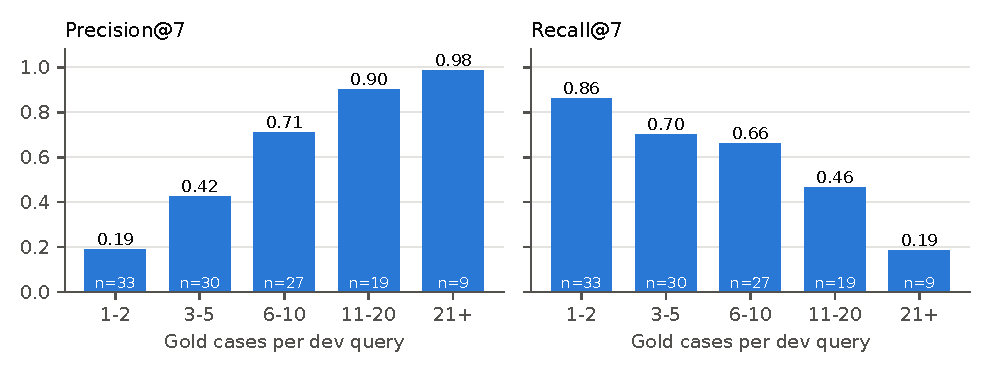
\includegraphics[width=0.85\linewidth]{fig_gold_size.pdf}
\caption{Phase 7 dev precision and recall by number of gold cases per query.}
\label{fig:p7gold}
\end{figure}

% ---------- Section 7.2, What the metrics do not measure ----------
Micro-F1@7 pools hits across queries, so the nine dev queries with 21 or more gold cases hold a third of all gold yet can yield few hits. Gold labels also record citation, not legal relevance: an uncited but relevant precedent counts as an error.

% ---------- Section 7.3, Limitations and next steps ----------
For Phase 7, the blend gains are a few hits, and one hit is worth about 0.0006 test F1. Our pool-level feature depends on the queries in a split, and both ranker and citing-context features are outside the Phase 1 models. The controls use one seed each, and the random start was tried at one learning rate for two epochs, so it bounds transfer only under this budget. Next we would score chunks of each candidate rather than one excerpt, so the neural stage can see text the lexical stage did not select, and test a mix of hard and random negatives.

% ---------- Section 7.4, Surprising findings ----------
In Phase 7, a position-only signal was worth more than any neural model: citing-context features added 17 test hits and the three rerankers about eight. The apparent collapse in recall on long queries disappeared once we accounted for the seven-slot cap. Random negatives were the biggest surprise: they raised standalone F1 by 0.061 and still lowered the blended score, so the better model alone was the worse component.

% ---------- Why techniques do or do not transfer (Section 7.1 or 8) ----------
Methods that suit our classification phases need not suit Phase 7. There, a label is predicted from one document's content, and pretrained representations can summarise it. PCR depends on a relation between two long documents, often verbatim reuse, which exact n-gram matching captures directly and a 1024-token excerpt only partly preserves.
